\documentclass[journal,10pt,twocolumn]{article}
\usepackage{graphicx, float}
\usepackage[margin=0.5in]{geometry}
\usepackage{amsmath, bm}
\usepackage{array}
\usepackage{booktabs}

\providecommand{\norm}[1]{\left\lVert#1\right\rVert}
\let\vec\mathbf
\newcommand{\myvec}[1]{\ensuremath{\begin{pmatrix}#1\end{pmatrix}}}
\newcommand{\mydet}[1]{\ensuremath{\begin{vmatrix}#1\end{vmatrix}}}

\title{\textbf{Line Assignment}}
\author{P Pavan Kumar}
\date{October 2022}

\begin{document}

\maketitle
\paragraph{\textit{Problem Statement} - Two sides of a rhombus ABCD are parallel to the ines y=x+2 and y=7x+3.1f the diagonals of the rhombus intersect at the point (1,2) and the vertex A is on the y-axis,find possible co-ordinate of A.}

\section*{\large Figure}

\begin{figure}[H]
\centering
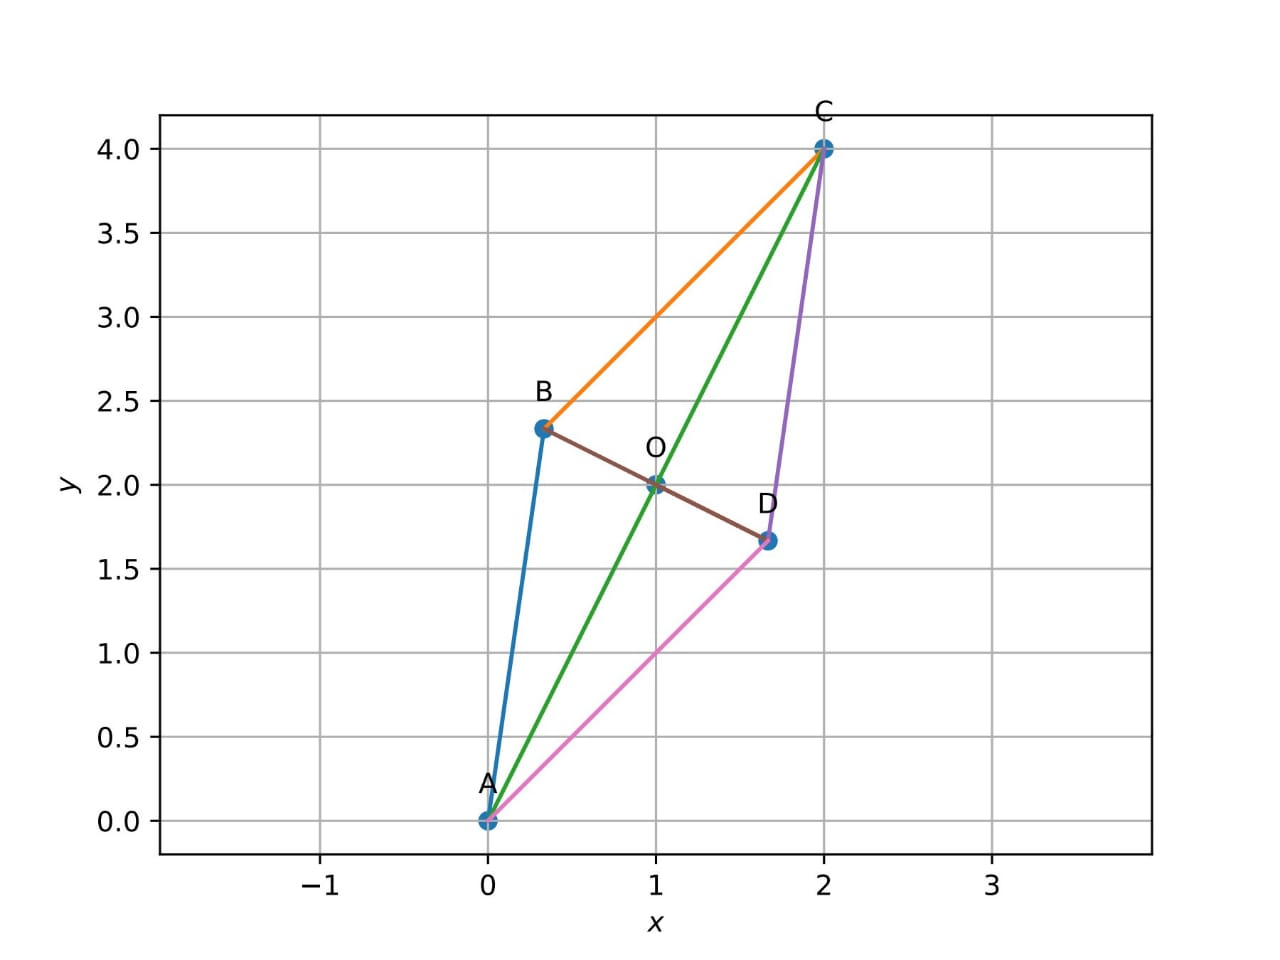
\includegraphics[width=1\columnwidth]{line.jpeg}
\caption{Diagonals intersect at point O(1,2)}
\label{fig:triangle}
\end{figure}
\section*{\large Solution}
The equation of the line1 y=x+2 and line2 y=7x+3.
\\we know that vector equation of the line is 
\begin{eqnarray}
 \vec{n^T}\vec{x}=c
\end{eqnarray}
The vector equation of the line1 and line2 is
\begin{eqnarray}
  (-1\hspace{2mm}1)\vec{x}=2
 \\(-7\hspace{2mm}1)\vec{x}=3
\end{eqnarray}
from above equations the direction vectors of AB and AD are 
\begin{equation}
\vec{m_1}=\myvec{1\\7}
\end{equation}
\begin{equation}
\vec{m_2}=\myvec{1\\1}
\end{equation}
To find the coordinate of A we use the parametric equation of the line 
\begin{equation}
\vec{X}=\vec{P}+\lambda\myvec{\frac{m_1}{\|m_1\|}+\frac{m_2}{\|m_2\|}}
\end{equation}
where
\begin{equation}
 \vec{x}=\vec{A}=\alpha\vec{e_2},
 \vec{P}=\myvec{1\\2}
\end{equation}
\begin{equation}
\alpha\vec{e_2}=\vec{P} + \lambda\myvec{\frac{m_1}{\|m_1\|}+\frac{m_2}{\|m_2\|}}
\end{equation}
multliplying the above equation with e1 transpose
\begin{equation}
\lambda = -1.178
\end{equation}
after finding the lambda substitute in the eq(12) slove for the equation for vertex A
\begin{equation}
\alpha\vec{e_2} = \vec{P} + \lambda\myvec{\frac{m_1}{\|m_1\|}+\frac{m_2}{\|m_2\|}}
\end{equation}
the vertex A is 
\begin{equation}
\vec{A}=\myvec{0\\0}
\end{equation}
The midpoint gives the vertex c
\begin{equation}
\vec{P} = \frac{\vec{A}+\vec{C}}{2}
\end{equation}

\begin{equation}
 \vec{C} = \myvec{2\\4}
 \label{eq4}
\end{equation}
the normal vectors are
\begin{equation}
\vec{n_1}=omat*\vec{m_1},
\vec{n_2}=omat*\vec{m_2}
\end{equation}
on sloving,we get
\begin{equation}
\vec{n_1}=\myvec{7\\-1},
\vec{n_2}=\myvec{1\\-1}
\end{equation}
the vertex B is the intersection of the lines 
\begin{equation}
  \vec{n_1^T}(\vec{x}-\vec{A})=0,
   \hspace{5mm}
   \vec{n_2^T}(\vec{x}-\vec{C})=0
\end{equation}
on solving, we get
\begin{equation}
    \vec{B}=\myvec{1/3\\7/3}
\end{equation}
the vertex D is the intersection of the lines 
\begin{equation}
   \vec{n_1^T}(\vec{x}-\vec{C})=0,
   \hspace{5mm}
   \vec{n_2^T}(\vec{x}-\vec{A})=0
\end{equation}
on solving, we get
\begin{equation}
    \vec{D}=\myvec{5/3\\5/3}
\end{equation}\\
 Hence the vertices of the rhombus are
 \begin{eqnarray}
 \vec{A} = \myvec{0\\0}\\
 \vec{B} = \myvec{1/3\\7/3}\\
 \vec{C} = \myvec{2\\4}\\
 \vec{D} = \myvec{5/3\\5/3}
\end{eqnarray}


\end{document}